\documentclass[12pt]{article}
\usepackage[utf8]{inputenc}
\usepackage{amsmath, amssymb, amsfonts, amsthm,  thmtools, graphicx, titlesec}
\usepackage[left = 2.5cm, right = 2.5cm, top = 2.5cm, bottom = 2.5cm]{geometry}
\usepackage[inline]{asymptote}

\usepackage[dvipsnames]{xcolor} 
\usepackage{hyperref}
\hypersetup{
    colorlinks=true,
    linktoc=all,
    linkcolor=RoyalBlue, 
    urlcolor=RoyalBlue
}

\everymath{\displaystyle}

\newcommand{\seperate}{\par\noindent\strut\hrulefill}

\newcounter{Problem}[section]
\newenvironment{prob}[1][]{\stepcounter{Problem} \newline\hyperlink{theproblem}{\textsf{\textbf{Problem \theProblem.}}}~ #1\rmfamily}{\medskip}

\newenvironment{lined-prob}[1][]{\stepcounter{Problem}\par\noindent\hyperlink{theproblem}{\textsf{\textbf{Problem \theProblem.}}}~ #1\rmfamily\color{Blue}}{\medskip\color{black}\seperate\bigskip}

\newenvironment{sol}[1][]{\newline\textbf{Solution.}~ #1\rmfamily}{\newline\null\hfill\blacksquare}{\medskip}

\newcounter{Altsol}[section]
\newenvironment{alt-sol}[1][]{\stepcounter{Altsol}\par\noindent\newline\textbf{Solution \theAltsol.}~ #1\rmfamily}{\newline\null\hfill\blacksquare}{\medskip}

\newcounter{AltsolMarking}[section]
\newenvironment{alt-sol-marking}[1][]{\stepcounter{AltsolMarking}\par\noindent\newline\textbf{Solution \theAltsolMarking.}~ #1\rmfamily}{\smallskip}

\usepackage[framemethod=TikZ]{mdframed}
\definecolor{Relic}{HTML}{00C030}
\mdfdefinestyle{mdRelicbox}{%
 linewidth=3pt,
 skipabove=12pt,
 frametitleaboveskip=5pt,
 frametitlebelowskip=0pt,
 skipbelow=2pt,
 frametitlefont=\bfseries,
 innertopmargin=4pt,
 innerbottommargin=8pt,
 nobreak=true,
 backgroundcolor=Relic!18,
 rightline=true,
 leftline=true,
 topline=false,
 bottomline=false,
 linecolor=Relic,
 }
\declaretheoremstyle[
 headfont=\sffamily\bfseries\color{RawSienna},
 mdframed={style=mdRelicbox},
 headpunct={: },
 postheadspace={0pt},
]{thmRelicbox}

\declaretheorem[style=thmRelicbox,name=Definition,numbered=no]{definition}
\definecolor{Alien}{HTML}{0050F0}
\mdfdefinestyle{mdAlienbox}{%
 linewidth=3pt,
 skipabove=12pt,
 frametitleaboveskip=5pt,
 frametitlebelowskip=0pt,
 skipbelow=2pt,
 frametitlefont=\bfseries,
 innertopmargin=4pt,
 innerbottommargin=8pt,
 nobreak=true,
 backgroundcolor=Alien!18,
 rightline=true,
 leftline=true,
 topline=false,
 bottomline=false,
 linecolor=Alien,
 }
\declaretheoremstyle[
 headfont=\sffamily\bfseries\color{RawSienna},
 mdframed={style=mdAlienbox},
 headpunct={. },
 postheadspace={0pt},
]{thmAlienbox}

\mdfdefinestyle{mdgreenbox}{%
 linewidth=3pt,
 skipabove=12pt,
 frametitleaboveskip=5pt,
 frametitlebelowskip=0pt,
 skipbelow=2pt,
 frametitlefont=\bfseries,
 innertopmargin=4pt,
 innerbottommargin=8pt,
 nobreak=true,
 backgroundcolor=Salmon!10,
 rightline=false,
 leftline=true,
 topline=false,
 bottomline=false,
 linecolor=Red,
}
\declaretheoremstyle[
 headfont=\sffamily\bfseries\color{RawSienna},
 mdframed={style=mdgreenbox},
 headpunct={. },
 postheadspace={0pt},
]{thmgreenbox}
\declaretheorem[style=thmgreenbox,name=Model,numbered=no]{model}

\newenvironment{prflem}[1][]{\newline\textit{Proof of lemma:}~ #1\rmfamily}{ \qed \newline}{\medskip}
\newenvironment{prfclaim}[1][]{\newline\textit{Proof:}~ #1\rmfamily}{ \qed \newline}{\medskip}


\title{IMMC 2020 : Flash sale}
\date{}
\author{TEAM NUMBER 20200901}

\begin{document}
\maketitle

\section{Summary}
\ \ \ \ Flash sale is an event where the owners of the stores aim to attract buyers by giving a huge discount on the products which couldn’t be easily found elsewhere. Obviously, people somehow want to save money by buying discounted products, and since there’s a limited amount of products, people stampede in to buy products and usually damage other products accidentally. It’ll be beneficial if we could alter the floor layout to minimize the damage caused by the buyers to the products, while keep being able to make a high potential profit or earning from the event. Hosting the flash sale with some specific layout will help increase the utility of the store, and increase the profit of the host. \newline\par
In this report, we identified how damage would be caused by the buyers by creating a model of chaos and messiness of floor layout, we showed that the popularity of a product depends on some properties of products; price (affordability), discount, demands, and brand. The messiness of the store depends on the popularity of the product that is selling in that store and the area of the store. To find the model of damage, we consider chaos instead of messiness. Chaos is defined around every path and corner. To compare two floor-layouts, we can simply compare the chaos of each model. \newline\par 
From the given layout, we analyze the chaos of the floor plan and found that the problem of this floor plan is the fact that there are too many corners, and corners contribute large value to chaos. It’s sensible that more corners cause more damage since when people are running uncontrollably, collision and damage will occur. In order to minimize the damage, we propose a new floor plan and provided proof that the proposed floor plan definitely gives small chaos and smaller potential damage from buyers’ clumsiness. \newline\par
The proposed floor plan uses the structure of the layout to force the people to walk systematically with an overall corner being reduced and with all corners having the products that can be damaged all removed. We can confirm that less collision will happen and as a result, lower potential damage dealt with the product. We consider all permutation of the department and choose the permutation giving the best result. Then for each department, we organize it the way that the store switch between the one with more messiness and the one with less messiness. This would make the damage be minimized and make this floor plan the best one we can generate. \newline

\newpage
\tableofcontents
\newpage

\section{Introduction} 
\ \ \ \ Flash sales are originally hosted to target consumers to shop at the local store in the holiday season or on the day people don’t go to work. Flash sales offer a huge discount to attract buyers in the expectation that the buyers will as well, spend on other regular price products. Undoubtedly, shoppers arrived at the entrance early and chaotically rush in. This chaos causes stampede, products damaging, and traffic jams. \newline \par
When flash sales are hosted, it’s important to capitalistically consider profit from the event, which is not only the money, but also the client bases, and brand advertising. The main aim of hosting the flash sale is to attract people to buy products, in this case, electronic appliances, and devices. The problem of hosting a flash sale is the potential damage from the accidental collision of the buyer against the products. \newline \par
We are proposing a way to organize the event venue of the electronic flash sale with a given product list to minimize the level of damage and increase the sales. 

\section{Restatement of Problem}
In this problem, we are required to do 4 main tasks:

1. Create a mathematical model that can calculate the competitive rate of each products from essential factors

2. Create a mathematical model that can calculate the damage of each floor plan layout

3. Place each products into the original floor plan layout

4. Create a new floor plan layout that decreases the potential damage and increase the expected sale profits

\noindent This can be further split into subtasks:

\noindent Task 1

a. Identify factors from information given in the products list, and researches that affects rivalry of the products

b. Calculate how each factor affect the rivalry in term of function

c. Calculate final competitive rate or rivalry based on the effects of each factor

\noindent Task 2

a. Calculate the competitive rate for each products using the created model

b. Calculate the number of people passing that products shelf

c. Calculate the chaotic value of each walkway / shopping lane 

d. Calculate the chaotic value of each intersection 

e. Calculate the overall chaos by considering the total chaotic value of the walkways and corners.

\noindent Task 3

a. Optimize the floor plan by organizing product stores position

\noindent Task 4

a. Try to reduce intersection which affects major part in chaos

b. Try to distribute people into distinct parts of shop to reduce chaos which is caused from many people being together in one place

c. Create model that satisfied the conditions

d. Use the model to calculate chaos which determines damage of the original floor plan layout

e. Use the model to calculate chaos which determines damage of the proposed floor plan layout 

\section{Variables}
\begin{tabular}{ | p{30mm} | p{130mm} | }
    \hline
    variables & meaning  \\\hline
    $P_{product}$ & Popularity of the product, Competitive rate, rivalry(depends directly on the product)\\\hline
    $P_{1,product}$ & Regular/Recommended price \\\hline
    $P_{2,product}$ & Flash sale price \\\hline
    $Q_{1,product}$ & Available quantity during flash sale  \\\hline
    $Q_{2,product}$ & Expected quantity to be sold during the event when the customer rating is 5\\\hline
    $Q'_{2,product}$ & Expected quantity to be sold during the event with concerning customer rating \\\hline
    $Cd_{product}$ & Rate of change of buying per 1\% change of price for the particular item \\\hline
    $Ed_{product type}$ & Elastic change of the demand of the particular product type (brand is not considered)\\\hline
    $\lambda$ $_{category}$ & Constant value indicating the effect of rating to the popularity \\\hline
    $M_{product}$ & Mess(chaos) of the shelf that contains particular product such as $M_{App-controlled\ robot}$] \\\hline
    $C_{path}$ & Chaos of the walkway\\\hline
    $C_{intersection}$ & Chaos of the intersection\\\hline
    $A$ & The effective area (see assumption(2))\\\hline


\end{tabular}
\newline
\newline
\newline
\noindent
\begin{tabular}{ | p{30mm} | p{130mm} | }
    \hline
    function & indicating  \\\hline
    $f$(rating) & Effect of rating to popularity \\\hline
    $g$(brand) & Effect of brand to demands \\\hline
    $f_2$(product) & the impact to level of damage depends on size of product \\\hline
    $h_1$(row of store$_i$, intersection$_j$) & Chaos of the intersection$_j$ that relates to the row of store$_i$ \\\hline
$h_2$($M_1,M_n$) & Chaos of the walkway($M_1,...,M_n$) \\\hline
\end{tabular}



\newpage
\section{General Assumption}
\ \ \ \ In order to use our mathematical model, we need to accept some assumptions including..
\begin{enumerate}
    \item Time wasted when the shoppers picking-up the products and when they are at the cashier are vanishingly small and can be neglected.
    \item There is only small amount of area which the customer have to be in, in order to be able to access the products. In reality, only finite number of people can be in that area. We assume that this area can be filled with infinite amount of people. So we assume this area to be the only area that are used to calculate the chaos(level of the damage of the product). This area is used to calculate the density of the customer who want that particular product. This area is called effective area( $0.955 m^2$)
    \item Every products has the same durability, so the damage dealt to the products only depends on their price and size.
    \item Damage is monotonically increased with respect to chaos. This allow us to construct the model that describe the chaos of the shop instead of the damage.
    \item Demand and price are linearly correlated. When the price is decrease, the demand will be increase. So the slope of the price-demand graph will be negative(both $Ed_{producttype},Cd_{product}$ are negative).
    \item Products abide by elastic economic model and elastic change of demand of products in the same type($Ed_{product type}$) are equal.
    \item The amount of products in flash sale is equal to the amount which are sold on non-promotion day, so all the products are expected to be sold out.
    \item Products rating, regardless of type, have the same effect to the demand of the products.
    \item Only the products on the side of the shelf can be accessed by the shopper so we can calculate damage by using only the perimeter of the shelf.
    \item All customers know about the layout beforehand. We can assume that the customers will spread overall the layout equally.
\end{enumerate}
 
\newpage
\section{Crucial factors}


\ \ \ \ The popularity of the product indicates the competitiveness, the rivalry of that products, the messiness, and the chaos which all resulted as damage. We need to consider all the factors that affect the popularity of the products and what property of can attract the customers. 
\newline

Firstly, we consider what will attract the shopper or what factors will affect the popularity of the product. Price and discount is the first one we need to consider. The lower the price the more the shoppers want to buy. The higher the discount the more they want to get this product. These two factors can be gathered from the given list. Brand and brand loyalty somehow play a big role in people decision. But we can't get this information so we considered it to be the same for all the products. Have you ever heard of the law of demand and supply? The less the products, the more rivalry there is for the customers Hence, the more the shoppers the higher the competitive tendency.
\newline

Secondly, to analyse damage value, we consider the chaos of the system to be monotonically correlated to damage value. Chaos can be identified from the effect of the popularity of the products and the store layout. For each products in the shop, the higher the popularity of the product is, the higher the competitive would be resulted in more damage value toward that product. Then we need to consider how damage can be caused from the products , we would assume that the weakness of the product is defined by its size and prize. Damaging more expensive products would obviously cause more damage. Since it's very difficult to calculate how fragile the product is. We will assume the products all have the same fragility. We also assume that the force done by the shoppers are equally distributed. This means that the bigger the product is, the higher probability of it being damaged, and the more force it would get from the shoppers.
\newline

Last but not least, when we consider the layout that influence the damage. We need to assume that when we consider a block of the store containing the products, the shopper can only access the products on the edge, meaning that only the edge of the block can be damaged. So we can calculate the potential damage of each block by measuring the edge or the perimeter if the block can be accessed on all four sides. For the area in front of the shelf, we assume that there's enough space for everyone to walk. In reality, only finite number of people standing in front of the shelf can access the products. However, in our model we would assume that every people in that area can access the products or in other words, can damage the products and we also assume that the messiness for the specific block is affected only by its own messiness and the ones adjacent to it.
\newline

\newpage
\section{Modeling and Calculation}
\par Rating influence people choice on choosing products. Higher rating products have more tendency to be bought. It’s obvious that the relation between rating and the tendency is monotonic: the higher rating is, the more likely it would be bought.We observed that the difference of 4-star and 5-star produce less impact than the difference of 1-star and 2-star rating. So it's reasonable to consider that popularity is correlated to the logarithmic scale of rating. We hereby use $log_5$(rating) with linear relation with some constant $k$. Since the product of the same category has similar usability, so the constant $k$ of the same category might be the same value, defined as $\lambda$ $_{category}$. So we can define $f$ as
\newline

\begin{definition}
$f$(rating)$\ \ \equiv\ \lambda_{category}\ log_5$(rating).
\end{definition}

From the assumption(8), the value of $\lambda$ $_{category}$ can be considered as $1$.

Therefore, we can have that 
\begin{center}
    $Q'_{2,product}=f$(rating)$Q_{2,product}$
\end{center}

\par 
It’s reasonable to have brand's influence factor in the model of demand of the product, since brand loyalty influence how buyer will choose the product. According to the definition of the price elastic of demand change of the particular product($Cd_{product}$) which is the percentage of change of the sales due to the change of the price of particular product and the assumption (5),(6),(7), we can conclude that 
\begin{center}
    $Cd_{product}=g$(brand) $Ed_{product type}$
\end{center}
But it is impossible to find the exact value of $Ed_{product type}$ from the stat. Because of the assumption(5), so we assume $Ed_{product type}=-1$. Unfortunately $g$ can’t be define from the given information, we now assume that no brands gain advantages from old clients. So we have 
\begin{definition}
$g$(brand)$\ \ \equiv\ 1.$ 
\end{definition}

As we assume that the $Q_{1,product}$ is the quantity that customer will buy in the usual event.
\par From the price elastic of demand formula and the assumption(7),

\begin{center}
    $Cd_{product}=(\dfrac{Q_{1,product}-Q_{2,product}}{P_{1,product}-P_{2,product}})(\dfrac{P_{1,product}+P_{2,product}}{Q_{1,product}+Q_{2,product}})$
\end{center}
It's also well known that the sign of $Cd_{product}$ is negative(from the assumption(5)). we get $Q_{2,product}$ as 
\begin{center}
    $Q_{2,product}=\dfrac{2Q_{1,product}}{1+\dfrac{Cd_{product}(P_{1,product}-P_{2,product})}{P_{1,product}+P_{2,product}}}-Q_{1,product}$
\end{center}

Since Rating affect buyers’ behavior
\begin{center}
    $Q'_{2,product}=f$(rating)$Q_{2,product}$
\end{center}
Then we can model the popularity of the product(competitive rate) as the ratio between Expected quantity sold during the event with customer rating concerning($Q'_{2,product}$) and the available quantity of the product($Q_{1,product}$).
\begin{model}
    $P_{product}=\dfrac{Q'_{2,product}}{Q_{1,product}}$
\end{model}


As we want to construct the model to describe the level of damage of each layout of the store. According to the assumption(4), we are going to construct the model to indicate the chaos of the product instead, since damage and chaos are correlated. First, we will define the \emph{store} as the only area that contains the particular item. Each item undergoes different amount of risk to be damaged since the chaos is related to many factors: 
\begin{enumerate}
    \item Popularity(competitive rate) of that product [$P_{product}$]
    \item Density of people struggling for that product at specific part of the store [$D_{product}$]
    \item The cost of that product[regular price $P_{1,product}$] (see assumption (10))
    \item The size of that product [$f_2$(product)]
    \item The durability of that product
\end{enumerate}
From the assumption(3) the durability of the product can be neglected. First, it's obviously true that when there are too many people in the small area, there will be very messy. The more density of people in the effective area (see assumption(2)), the more chaotic the store is. In addition, if the popularity of that product is high, the competitive rate of customer is also high, lead to more Chaos in the system. Therefore, in order to calculate chaos of the store, we assume that the relation between the chaos caused by the store and both popularity and the density of customer is linear. Since the value of each product is different, the damage caused by the product is then relates to the cost of that product. It's also a common sense that the chaos depends directly to the physical size of the product. Finally, we can calculate the chaos caused by the store of the product

\[M \equiv D_{product} \times M_{product,i}\times P_{1,product} \times f_2 (product)\times constant\ of\ the\ correlation\]

Let A represents effective area which already mentioned in assumption(2) and $f_2$ maps product the store sell, to the contribution to mess of the store, determine the size of the product. Let a representative of amount of item the store contain is $q_i$, so $P_{product} \times q_i$ indicate the predicted number of customer that will come to struggle this product. 
\medskip Therefore, $D_{product}=\dfrac{P_{product} \times q_i}{A}$

Then we define $M_{product}$ as 
\begin{definition}
$M_{product} \equiv 1+ \dfrac{M}{M_{sum}}$
\end{definition}
,where $M_{sum}$ is the sum of all M value of all store in the shop.
This make $M_{product}\in (1,2)$

Now we have the $M_{product}$ indicate the chaos value caused by the particular store of product.Now consider the row of store and each store's $M_{product}$. Let the $M_{product,i}$ be it's $M_{product}$. As see in figure 1.
\begin{center}
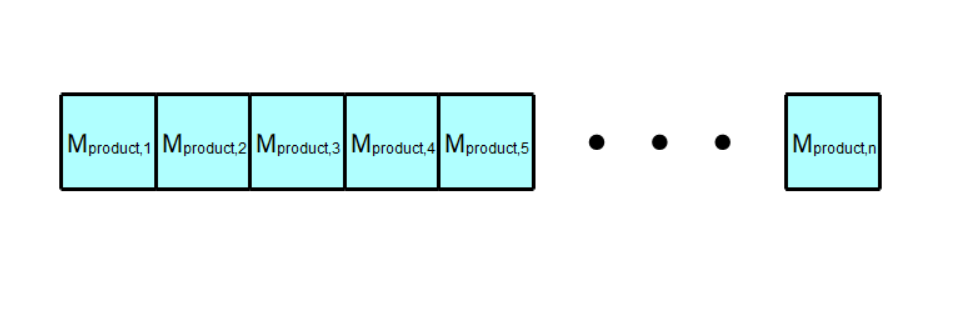
\includegraphics[width=\textwidth]{fig3.PNG}
Figure 1
\end{center}


Since when the store is very mess, it's neighbours will be impacted. So we say that chaos of a walkway that pass through the store is determined by itself and its neighbours Mess. We say that the chaos is the product of itself and its adjacent member because the shoppers don't just increase the messiness to only the store, but to the area(walkway). Chaos of the walk way is formally defined as

\begin{model}
    $C_{path}=\displaystyle{\sum_{i=1}^{n}\ M_{product,i-1}\times M_{product,i}\times M_{product,i+1} }$
\end{model}
,where $M_{product,0}=M_{product,n+1}=1$

Then we define function 
\begin{definition}
$h_2$($M_1,M_n$) $\equiv$ the function that calculate the $C_{pathM_1...M_n}$.
\end{definition}
For instance, the walkway of figure 2 has chaos value $C_{path}$ equal to $[M_1M_2+M_1M_2M_3+M_2M_3M_4+M_3M_4M_5+M_4M_5M_6+M_5M_6]+[M'_1M'_2+M'_1M'_2M'_3+M'_2M'_3M'_4+M'_3M'_4M'_5+M'_4M'_5M'_6+M'_5M'_6]$ and $h_2$($M_1,M_6$)$=[M_1M_2+M_1M_2M_3+M_2M_3M_4+M_3M_4M_5+M_4M_5M_6+M_5M_6]$.In this figure, we use $M_i$ to represent $M_{product,i}$.
\begin{center}
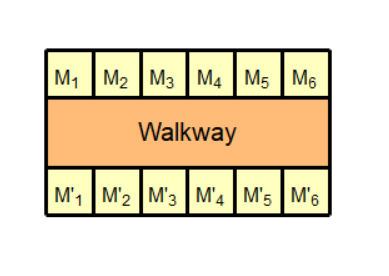
\includegraphics[]{fig1.PNG}

Figure 2.
\end{center}

Next, the mess of the intersection is caused by the shopper walk along the row of store, that is connected to the intersection. The red and green point in the Figure 3 indicate two different types of the intersection. Next we will use $M_{product,i}$ to indicate both chaos value of the product$_i$ and the store that contains p;product$_i$. 

\begin{center}
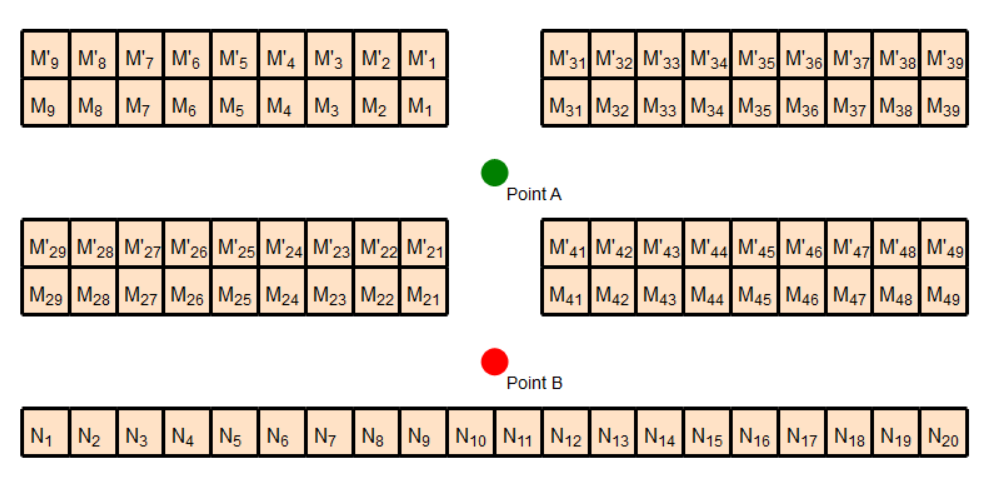
\includegraphics[width=\textwidth]{fig2.PNG}
Figure 3
\end{center}

For the green point, we know that the more people come from 4 directions([$M'_1M_1$ or $M_{31}M'_{31}$], [$M_{31}M_{39}$ or $M'_{41}M'_{49}$], [$M_1M_9$ or $M'_{21}M'_{29}$] and [$M'_{41}M_{41}$ or $M_{21}M'_{21}$]) that connected to this point. So the mess of this intersection point is related to how many shopper come to this point. But customers can only go to this point if customers walk(run) through these 4 walkway. So the chaos of the intersection is directly related to how mess of each store along the walkway. In addition, two products at the corner(adjacent to the intersection) also impact the chaos of the intersection. Because the intersection is where customer will brake, slow down, change the direction, these kind of action can be easily cause the collision of the customer who come from different direction. This collision will affect the store that is adjacent to the intersection. So if these two store which adjacent to the intersection have high value of mess point($M_{product}$), there will be very messy. So we define the function $h_1$(row of store$_i$,intersection$_j$) as the function that calculate the chaos value that generated by the store in the row of store$_i$, which belong to the particular walkway that is connected to the intersection$_j$.
So we define function
\begin{definition}
$h_1$(row  of store$_i$,intersection$_j$)$\equiv \displaystyle{M_{product,1} \times M_{product,2} \times [{\sum_{M_{product,i}\in \mathbb{W}} M_{product,i}}]}$
\end{definition}
\par where $\mathbb{W}$ represent a set of the store in the row of store$_i$ that is connected to the intersection$_j$, the $M_{product,1}$ and $ M_{product,2}$ are adjacent store and the $M_{product,1}$ store connected to the intersection$_j$.

So we define the chaos of the intersection as 

\begin{model}
    $C_{intersection_j}=\displaystyle{\sum_{row\ of\ store_i\in \mathbb{D}}} h_1$(row of store$_i$,intersection$_j$)
\end{model}

Where we define $\mathbb{D}$ as the set of all row of store connected to that intersection$_j$ 

For instance,
\begin{enumerate}
    \item[] $h_1$(row of store$_{M_1...M_9}$,intersection$A$)$=M_1M_2(\sum_{i=1}^{9}M_i)$
    \item[] $C_{intersection_A}=\sum_{i=0}^{3}(M_{i1}M'_{i1}(M_{i1}+M'_{i1})) + M_1M_2(\sum_{i=1}^{9}M_i) + M_{11}M_{12}(\sum_{i=1}^{9}M_{1i}) + M'_{21}M'_{22}(\sum_{i=1}^{9}M'_{2i}) + M'_{31}M'_{32}(\sum_{i=1}^{9}M'_{3i})$
    \item[] $C_{intersection_B}=\sum_{i=2}^{3}(M_{i1}M'_{i1}(M_{i1}+M'_{i1}) + M_{i1}M_{i2}(\sum_{j=1}^{9}M_{ij})) + N_9N_{10}(\sum_{i=1}^{10}N_i) + N_{11}N_{12}(\sum_{i=11}^{20}N_i)$
\end{enumerate}

Finally we calculate the chaos value of the shop's layout by adding all $C_{intersection_j}$ for all intersection$_j$ in the shop's layout. This chaos value of the shop's layout can be used to compare which shop's layout will able to cause the highest damage to the product. The shop with high chaos value will able to cause high damage to the product. So our goal is to find the layout of the shop that can make the chaos value to be the lowest.

\newpage
\section{Solutions and Suggestions}
\textbf{Placing products into original floor plan layout}
\newline
\par Since the factors affecting the damage for this fixed floor plan is placing the products. The popularity of the product indicates the competitive indicates the damage. Since for each store, the number of people passing it is not equal. The store that's placed nearer to the front (cashier-entrance-exit zone) have more probability to be passed by bigger number of people. We need to place the products with high popularity on the low traffic place, the further one to the back. We can place the department which can be seen in figure 4 
\newline

\begin{center}
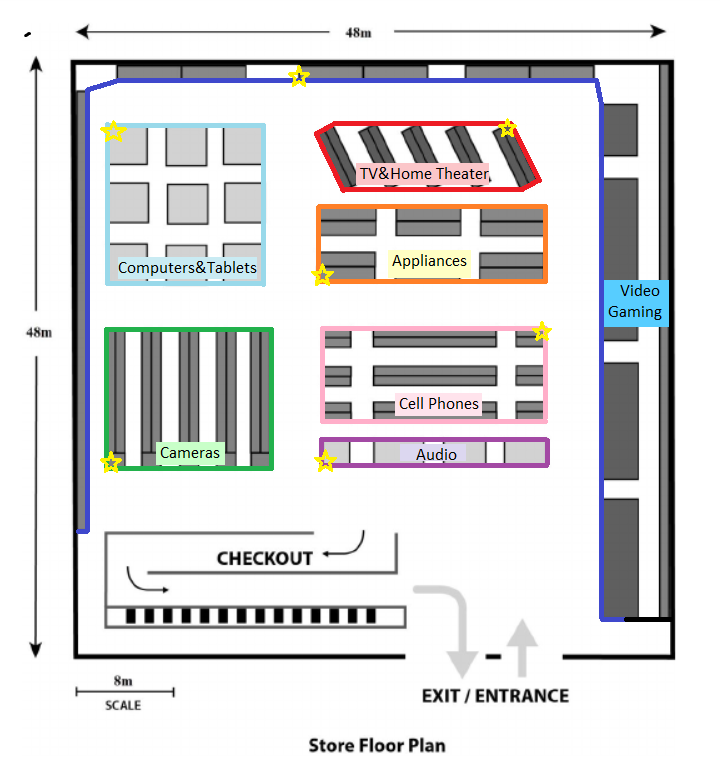
\includegraphics[width=0.6\textwidth]{fig4.4.PNG} 
\end{center}
\begin{center}
Figure 4.
\end{center}

\par The above figure represents about the strategy of ordering departments in the original floor plan layout. The plan consists of seven departments and seven stars representing the highest rating product of the department including Sport Wireless Earbud Headphones in Audio department, 5.1cu ft Freestanding Gas Range, Stainless Steel from Appliances department, Mirrorless Camera with Lens from Cameras department, Wireless Wearable Speaker - Black from Cell Phones department, 2-in-1 14" Touch-Screen Chromebook, Intel Core i3, 4GB RAM, 128GB from Computers\&Tablets department, 55" 4K UHD HDR Smart OLED TV, A8G Series from TV\&Home Theater department, and lastly, 32GB Console - Gray Joy-Con + 2 more items from Video Gaming department. Among all of the products, we found that the most popular one is the Mirrorless Cameras with Lens. Our strategy is to place the higher rating products further from the cashier-entrance-exit zone to prevent the chaos from people grabbing the valuable products. Moreover, the highest rating products of each department need to be placed far from each other enough so that they won't cause chaos, but not too far so that people can still walk around to see another products to increase the sales. \newline
\noindent \textbf{Creating new floor plan layout}
\newline
\par Since the factors that we consider having affect on the damage caused by the shoppers, for the layout one of them is the corner. We will try to build the layout with least corner possibly none. Our model will try to make them walk through a straight pathway so that there's no corner. Then we can see that having all of them walking in one pathway might not be the best way. Distributing them into many pathway might help. But if we need to distribute them into more than one pathway and then have a hole for them to pass through to get to another path, this would cause chaos and collision too. Our idea is to have them all walking in one straight way each pathway independently.
\newline
\begin{center}
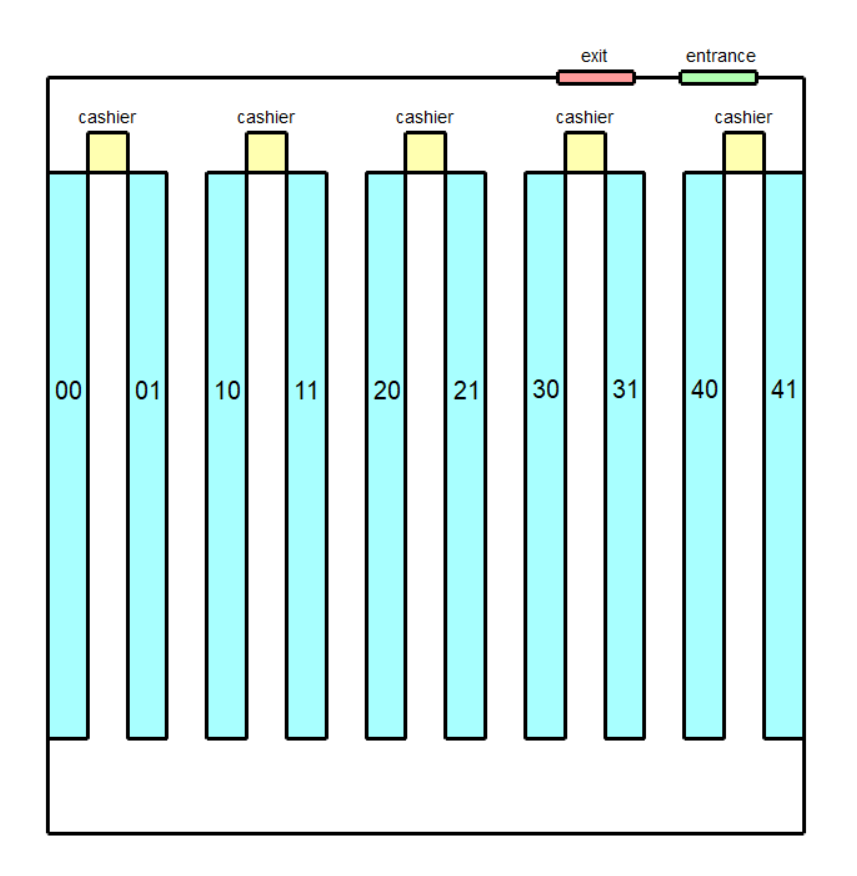
\includegraphics[width=0.6\textwidth]{fig4.1.PNG} 
\end{center}
\begin{center}
Figure 5.
\end{center}

\par From the layout, we can see that the customer will walk in through the entrance (green block in fig.4) then they would be forced to separate and enter each of the space between the shelf. The products can be accessed only from the cashier side, meaning that when the customers arrive, they will need to walk in pass the cashier through the space between each shelf, then make a u-turn to go the space that have the cashier at their ends. This layout has no corner with products, meaning reduced collision. Having them walking straight would reduce the orderlessness that occur in the original layout. After they finish picking up products they will need to pay at the cashier and then walk out at the exit. Even though the area behind that the cashier that's connected to both the entrance and the exit, the chaos would be really bad, but since there's no products to be damaged there, no damaged would be caused.
\newline

\par Then we need to place the products into the shelf. We would define each of the two shelves that can be accessed from the same space as a block. A block would contain a walkway having a cashier at its end, two shelves on the left and the right. 
\newline

\par We then need to make as much block as possible to distribute the people to minimize the chaos. Since each block is independent to the others meaning that people can't go from one block to another so each block would need to contain all the products that the customer would need. Since the products having least amount has the amount of five. We can make five blocks. (can be seen in fig.4) We expected that the alignment of the product store, and the chaos of each shopping lane to be comparable since it will equally distribute people into every lane and lower the overall chaos of the shopping hall.
\newline

\begin{center}
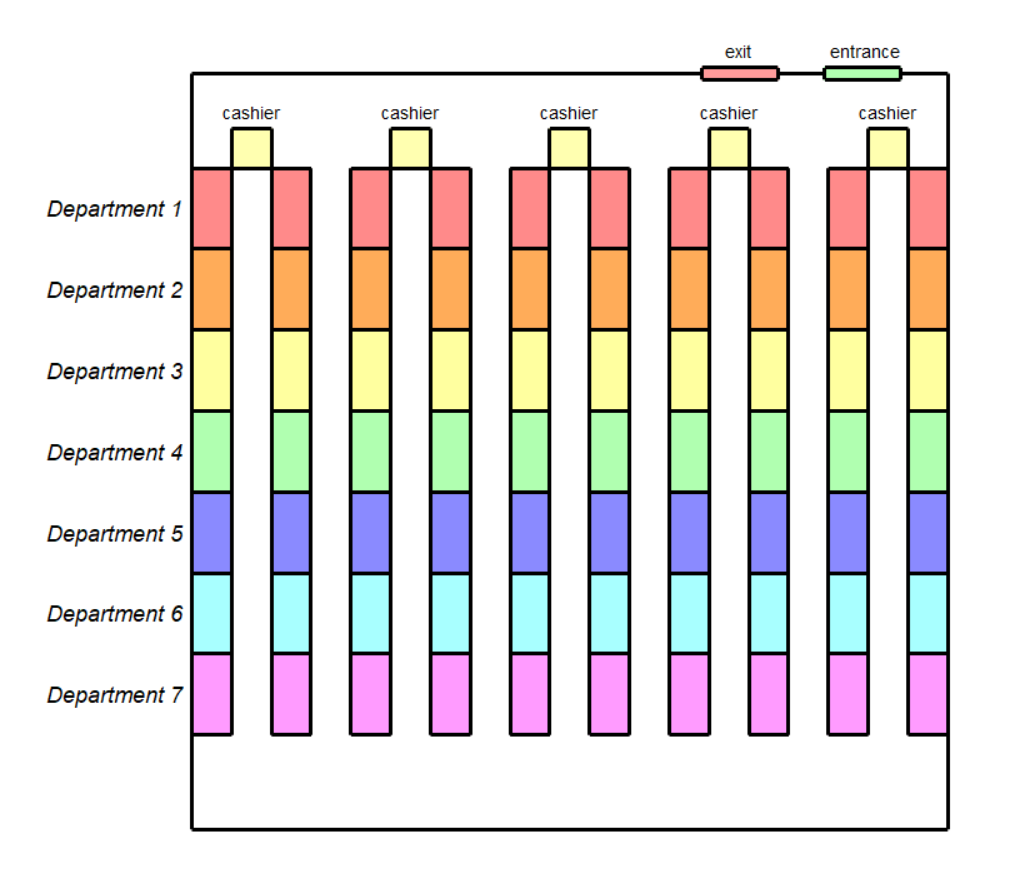
\includegraphics[width=0.7\textwidth]{fig4.2.PNG} 
\end{center}
\begin{center}
Figure 6.
\end{center}

\par Then we need to find a way to place the products. Since the products from the same department need to be placed together. We would permute the department and choose the best permutation of the department. For each permutation, we would add the products according to the permutation. (please see fig.5 for better understanding). For each department we would try to switch the products in the way that for each side of the block shelf, the messiness of the sequence of the products would be small then big then small continuously, because our model consider the messiness point as the product of its own messiness and the adjacent ones. 
\newline

\par Since calculating all the permutation by hand would be such an enormous thing to do within limited time. We would solve the problem by writing a computer program to permute and then calculate the total damage (messiness) of all the permutation and then pick the best one with minimal damage calculated based on the layout and the mathematical model.
\newline

\par Then our code will generate the products list that needed to be placed in each block separately. Then the store manager can place the products according to it to minimize the damage.
\newline

\par From our code we get that the permutation that give the optimal solution with the minimum damage is the layout below

\begin{center}
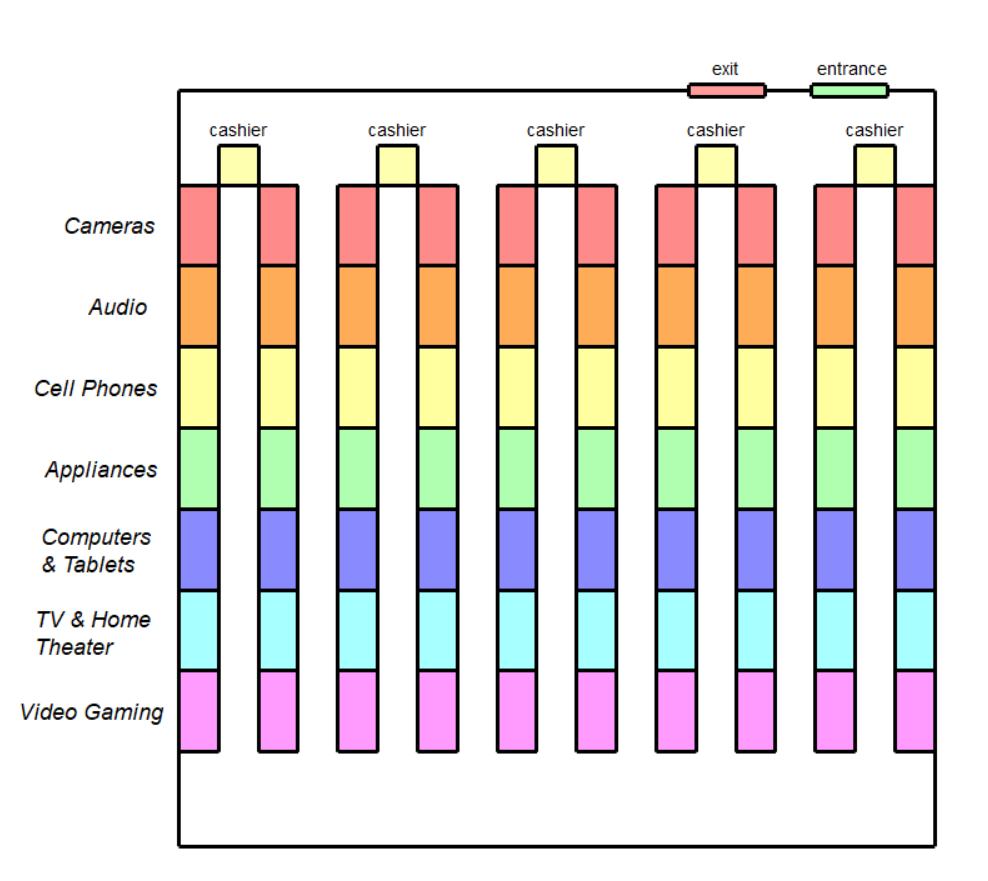
\includegraphics[width=0.7\textwidth]{fig4.3.PNG} 
\end{center}
\begin{center}
Figure 7.
\end{center}

\newpage
\section{Floor plan}
\begin{center}
    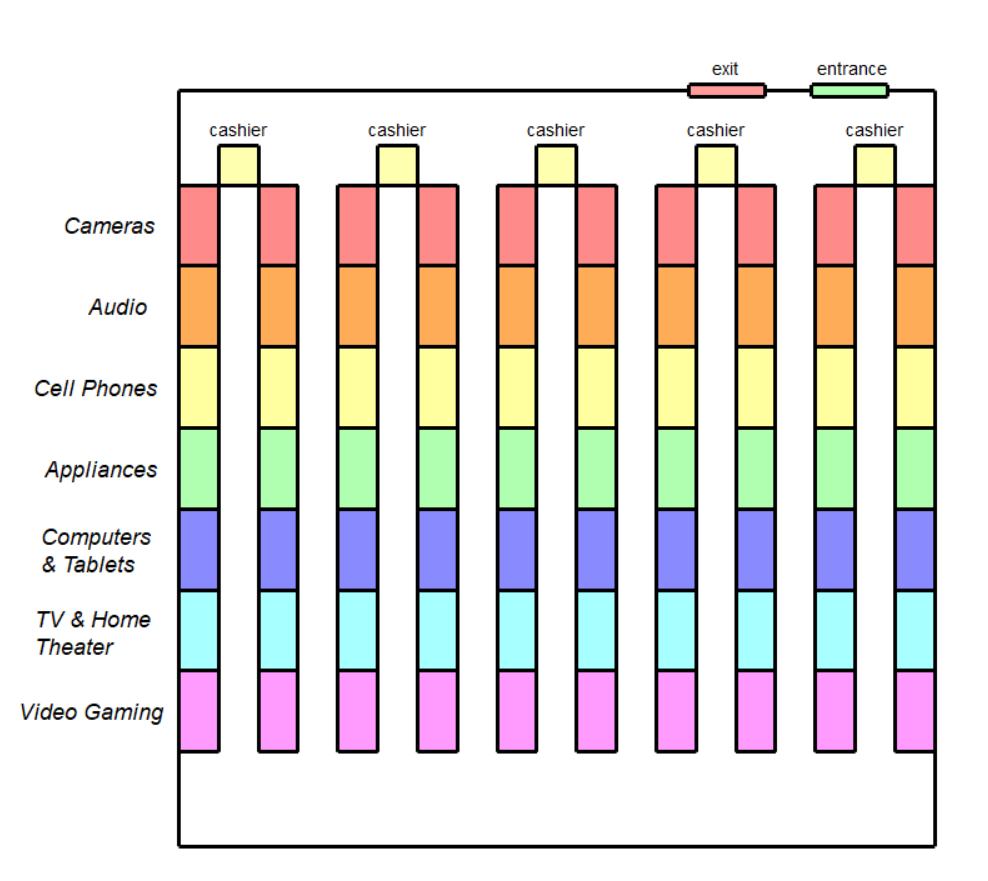
\includegraphics[width=\textwidth]{fig4.3.PNG}
\end{center}

First we define ProductID of each product by iterating over all the element in the given dataset and we let the first one be the product with ProductID = 0, and the next one having ProductID = 1 and so on.
\newline \par
Five shelves in above figure are organized identically following this given rule.
\newline
\par For every left shelf, we place product by this following sequence (from bottom to top)
\newline
42, 39, 33, 38, 35, 32, 45, 44, 18, 14, 13, 10, 12, 23, 20, 29, 28, 25, 27, 6, 7, 2, 1, 54, 55, 53, 64, 67, 69, 65, 60, 56, 62, 46, 48, 49, 85, 72, 76, 74, 78, 82, 80, 98, 92, 96, 95, 105, 99, 103, 104, 106, 114, 117, 116, 118, 111, 112, 86, 89, 87, 121, 122, 125, 126, 132, 130, 
\newline \par
For every right shelf, we place product by this following sequence (from bottom to top) \newline
41, 40, 34, 37, 36, 31, 43, 16, 17, 15, 9, 11, 21, 19, 22, 30, 24, 26, 5, 4, 8, 3, 0, 52, 51, 70, 63, 68, 66, 57, 59, 58, 61, 47, 50, 84, 75, 73, 71, 77, 81, 79, 83, 91, 97, 94, 93, 102, 101, 100, 108, 107, 119, 115, 120, 109, 110, 113, 88, 90, 124, 123, 129, 127, 128, 131, 133, 

\begin{center}
    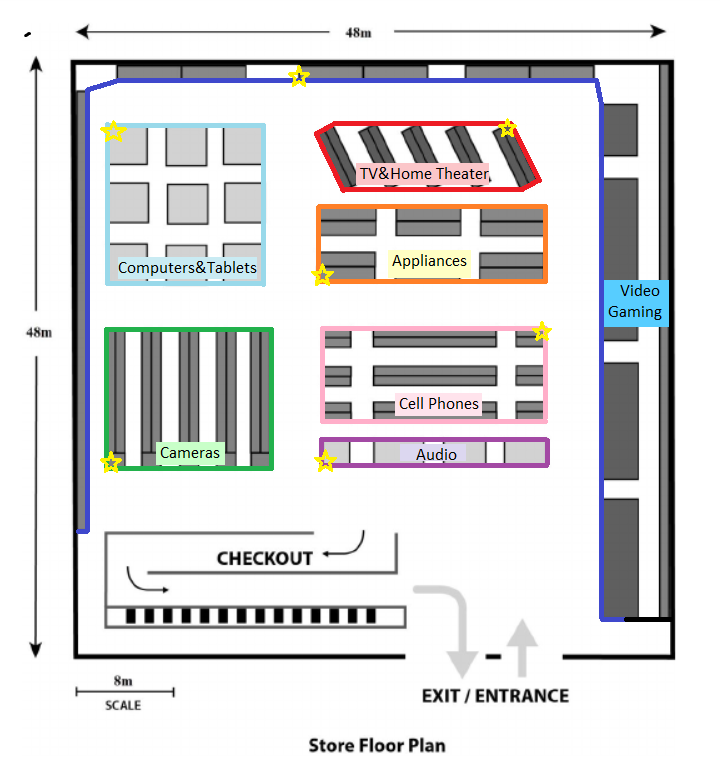
\includegraphics[width=\textwidth]{fig4.4.PNG}
\end{center}

legend - star indicates the most popular products in the department
\newpage
\section{Analysis of Our Model}
\ \ \ \ Since the layout we get is from the permutation that the code generated. It would be considered as the best one among other permutation. 
\newline

\textbf{Strengths}
\begin{itemize}
    \item Our new floor plan layout is better than the original one
        \newline
        \ \ \ \ - expected damage is lowered
        \newline
        \ \ \ \ - potential profit remains the same
        \newline
        \ \ \ \ - people will walk in more orderly way (straight line with no corner having products)
    \item Our new products layout is the best for this floor plan layout
        \newline
        \ \ \ \ - tested among all possible permutations
        \newline
        \ \ \ \ - people are ideally randomly distributed to all lanes
        \newline
        \ \ \ \ - each lane has all types of products
    \item Our layout is easy-to-use
        \newline
        \ \ \ \ - our layout contains floor plan and specific location to place the products
\end{itemize}

\textbf{Limitation}
\begin{itemize}
    \item The floor plan layout relies on mathematical model
        \newline
        \ \ \ \ - this layout is optimal only for this mathematical model
        \newline
        \ \ \ \ - changing in mathematical model might make this layout not optimal
\end{itemize}

\newpage
\section{Compare models}
\ \ \ \ As we already construct the model and mathematical model that can calculate the chaos of the shop's layout, we are going to show that the created model is proper and can cause less damage to the products. 
\newline \par
Consider Figure 5.1 \& Figure 5.2
\begin{center}
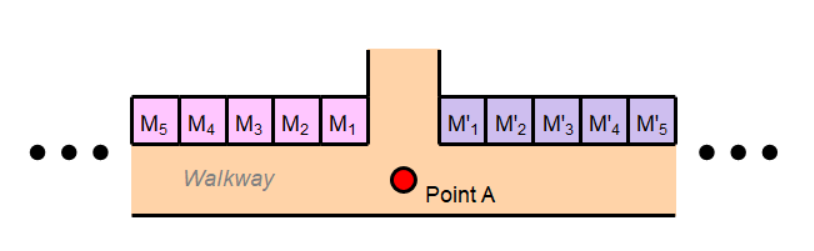
\includegraphics[width=\textwidth]{fig5.1.PNG}
Figure 8.1
\end{center}
\begin{center}
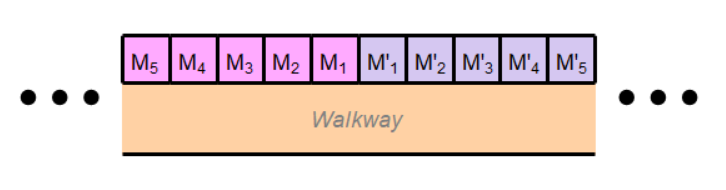
\includegraphics[width=\textwidth]{fig5.2.PNG}
Figure 8.2
\end{center}
\par
Now we are going to calculate the overall chaos value (that is related to store $M_1,M_2,\hdots,M_n$ and $M'_1,M'_2,\hdots,M'_n$) of the figure 8.1 and compare with figure 8.2.

The chaos of the figure 8.1 includes chaos of the walkway(caused by $M_1,M_2,\hdots,M_n$ and $M'_1,M'_2,\hdots,M'_n$) and the chaos of the intersection$_A$(caused by the row of store$_{M_1,M_2,\hdots,M_n}$ and row of store$_{M'_1,M'_2,\hdots,M'_n}$). The chaos of figure 8.2 contains only the chaos of walk way that is related to row of store$_{M_n,M_{n-1},M_{n-2},\hdots,M_2,M_1,M'_1,M'_2,\hdots,M'_n}$
Let the intersection$_A$ abbreviate as \emph{A}.
\newline
\newline
First, we calculate the chaos of the walkway.
\begin{enumerate}
    \item[] chaos of walkway$_{M_1,M_2,\hdots,M_n}=h_2$($M_1,M_n$)
    \item[] chaos of walkway$_{M'_1,M'_2,\hdots,M'_n}=h_2$($M'_1,M'_n$)
    \item[] chaos of walkway$_{M_n,M_{n-1},\hdots,M_2,M_1,M'_1,M'_2,\hdots,M'_n}$=$h_2$($M_n,M'_n$)
\end{enumerate}
\par
Then, we calculate the chaos of the intersection$_A$
\begin{enumerate}
    \item[] chaos of the intersection$_A=h_1$(row of store${_{M_n,M_{n-1},\hdots,M_1}}$,intersection$_A$) + $h_1$(row of store${_{M'_1,M'_2,\hdots,M'_n}}$,intersection$_A$)
\end{enumerate}
Let's define $H \equiv $ $h_1$(row of store$_{M_n,\hdots,M_1}$,\emph{A})
and 
$H' \equiv $ $h_1$(row of store$_{M'_n,\hdots,M'_1}$,\emph{A})

So it's enough to prove that 
\begin{center}
    $H$ + $H'$ + $h_2$($M_1,M_n$) + $h_2$($M'_1,M'_n$) $>$ $h_2$($M'_1,M'_n$)
\end{center}

\par
Let $\mathbb{M}$ be the set of all $M_{product}$
From $M_{product} \in (1,2)$, so for all $a,b,c \in \mathbb{M}$
We get that $a+b>1+1=2>c$.

Since $M_1,M_2,M'_1,M'_2\ \in \mathbb{M}$, then $M_1+M_2>M'_1$ and $M'_1+M'_2>M_1$
We get that
$M_1+\hdots+M_n\ >\ M_1+M_2\ >\ M'_1$ $\iff M_1M_2(M_1+\hdots+M_n)>M_1M_2M'_1$
\newline Therefore, we have
\begin{center}
    $M_1M_2(M_1+\hdots+M_n)>M_1M_2M'_1$ and $M'_1M'_2(M'_1+\hdots+M'_n)>M'_1M'_2M_1$
\end{center}

\begin{center}
$H$ + $H'$ $> M_1M_2M'_1+M'_1M'_2M_1$ 
\end{center}
\begin{center}
$\iff$
\end{center}
\begin{center}
$h_2$($M_1,M_n$) $ - M_1M_2+h_2$ ($M'_1,M'_n$) $ - M'_1M'_2+H$ + $H'$ $ > M_1M_2M'_1+M'_1M'_2M_1 + h_2$($M_1,M_n$)$ - M_1M_2+h_2$($M'_1,M'_n$)$ - M'_1M'_2$
\end{center}
\par
So $ h_2$($M_1,M_n$)$ + h_2$($M'_1,M'_n$)$ + H$ + $H'$ $ > h_2$($M'_1,M'_n$) as desired.
\par So we can conclude that if there exist two row of store connect to the same intersection, the chaos that related to all the store in these two row of store will be reduced when these two row of connect to each other. 
\par
In the similar way of proof, we can get that the chaos value related to store $M_1,M_2,\hdots M_n,M'_1,\hdots M'_n$ in figure 9.1 will be larger than in that the figure 9.2

\begin{center}
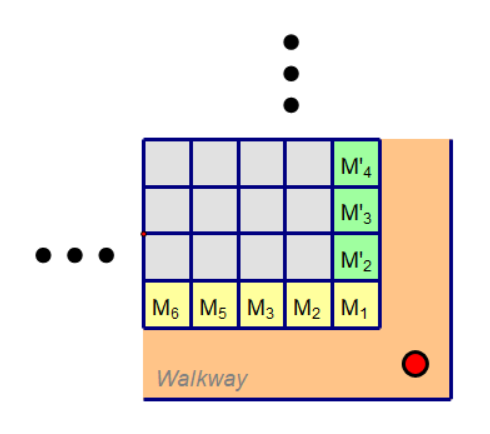
\includegraphics[width=0.7\textwidth]{fig6.1.PNG}
\end{center}
\begin{center}
Figure 9.1
\end{center}
\begin{center}
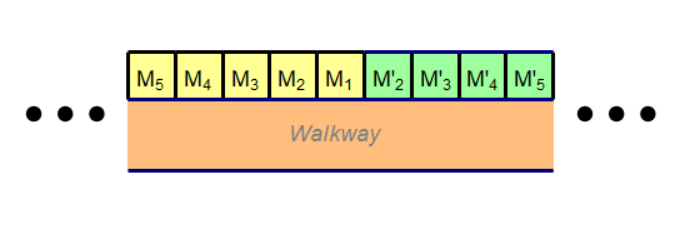
\includegraphics[width=\textwidth]{fig6.2.PNG}
\end{center}
\begin{center}
Figure 9.2
\end{center}

Therefore, if we connect two roles of store that either connect to the same intersection or perpendicular to each other(like figure 9.1) to be new long straight row of store, the new row of store will have lower chaos value.


When we consider the given layout, we can see many corners, which make the chaos of shop's layout to be high. We are going to show that it's able to find a chain from the layout such that this chain cover all the stores,in the condition that the same product type is adjacent, the same category is adjacent and the same department is adjacent. So if we use this new chain, called model \emph{L} to form a new layout of shop, like one long straight row of the store. [See figure 10 for an example of the chain], this long straight row(model \emph{L}) will has lower chaos value than the given layout as shown above.
\newline

Now we consider the model \emph{L}. As we have already mentioned(in solution and suggestion) that we use computer program to compile the permutation of the product in the linear layout, we get that the chaos value will be lower if there are more shopping lines of shelves.

Therefore, the given layout has higher chaos value than model \emph{L} and model \emph{L} has higher chaos than our proposed model, so the given layout also be more orderless and chaotic than our proposed model. Although we split the shopping mall into several shopping lines, we distribution all of the products to every shopping line equally to make sure that the spenders get the best shopping experience and choices to make, which will absolutely increase the spending probability and provide the host with more profits. Unfortunately, there exists a product which only is 5 item in quantity, so we can maximally split the shopping lanes into 5 lanes without losing economical advantages (in the amortized sense). From the computed data, we see that 5 lanes of shopping shelves provides good-enough result: doesn't significantly different to 6 or more lanes.

\begin{center}
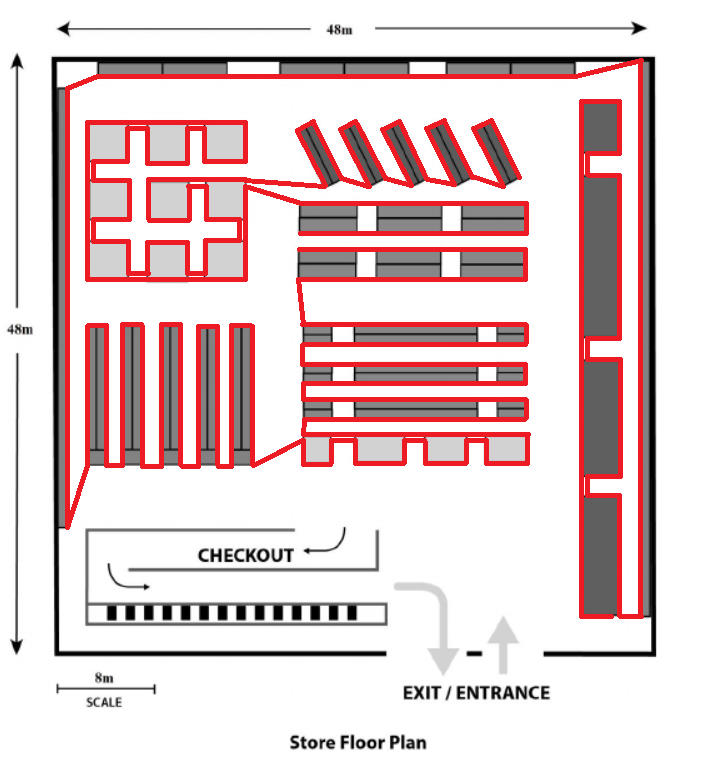
\includegraphics[width=\textwidth]{fig6.PNG}
Figure 10.
\end{center}
\newpage
\section{Appendix}
\begin{tabular}{p{40mm} p{100mm}}
    Chaos & The messiness, disordering caused by struggling of the customers or the collision of the customer at the intersection \newline\\
    Chaos value & The specific value that indicates chaos. High number of chaos value determine high chaotic condition of the area \newline\\
    Competitive rate & The ratio between0 available amount of products to the needs of customers. This value also indicates how famous/popular the product is \newline\\
    Damage & Physical damage happened to the product that might be caused during the flash sale event \newline\\
    Demand  & Economic value that indicates the need of product to the market(customers)\newline \\
    Department & Major division of the products \newline\\
    Intersection & The point where two pathway cross each other \newline\\
    Popularity & Thing that used to indicate how famous the product is ,define similarly as the competitive rate \newline\\
    Product & The particular item that is specific in brand, type, category, department, and its economic properties  \newline\\
    Product type & Sub category or minor grouping of products\newline\\
    Row of store & A consecutive line of shelves  \newline\\
    Shelf & The construction that hold up the product to show to customer as a store \newline \\
    Store & A particular shelf that contains only one specific product \newline\\
    Walkway & The area in front of the store that the customer can walk through and pick the product : The path along the row of the store that customer can walk \newline\\
\end{tabular}

\newpage
\section{Reference}
\ \ \ \ 
\texttt{[1] Aday, James Brian. “Competitive Advantage or Market Saturation: An In-Depth Comparison of Flash-Sale Sites Through Content Analysis.” Taylor; Francis, Nov. 2014,}
\url{https://www.tandfonline.com/doi/abs/10.1080/19368623.2014.905815}.

\texttt{[2] Chen, ChenCheng-Hao. “Exploring Electronic Word-of-Mouth (EWOM) in The Consumer Purchase Decision-Making Process: The Case of Online Holidays – Evidence from United Kingdom (UK) Consumers.” Taylor; Francis,}
\url{ https://www.tandfonline.com/doi/abs/10.1080/10548408.2014.956165.}

\texttt{[3] Chi, Hsin  Kuang. “The Impact of Brand Awareness on Consumer Purchase Intention: The Mediating Effect of Perceived Quality and Brand Loyalty.” The Impact of Brand Awareness on Consumer Purchase Intention: The Mediating Effect of Perceived Quality and Brand Loyalty, Feb. 2009,} \url{http://203.72.2.146/bitstream/987654321/27159/1/The+Impact+of+Brand.pdf}.

\texttt{[4] Chinthalapati, Raju. “Dynamic Price in Retail Market.” Learning Dynamic Prices in MultiSeller Electronic Retail Markets with Price Sensitive Customers, Stochastic Demands, and Inventory Replenishments - IEEE Journals; Magazine,}
\url{https://ieeexplore.ieee.org/abstract/document/1603740}.

\texttt{[5] Day, George S. "A Two-Dimensional Concept of Brand Loyalty." SpringerLink. Springer, Berlin, Heidelberg, 01 Jan. 1976. Web. 03 Apr. 2020.}
\url{https://link.springer.com/chapter/10.1007%2F978-3-642-51565-1_26}.

\texttt{[6] Dwyer, Ehrenberg, "Consumers' Trust in a Brand and the Link to Brand Loyalty." Journal of Market-Focused Management. Kluwer Academic Publishers, 01 Jan. 1991. Web. 03 Apr. 2020.} \url{https://link.springer.com/article/10.1023/A:1009886520142}

\texttt{[7] Gartner,“Optimal Traffic Assignment with Elastic Demands: A Review Part I. Analysis Framework.” Traffic Assignment on Elastic Demands, 1 May 1980,}
\url{https://pubsonline.informs.org/doi/abs/10.1287/trsc.14.2.174}.

\texttt{[8] Jacoby, Jacob,“Brand Loyalty Vs. Repeat Purchasing Behavior - Jacob Jacoby, David B. Kyner, 1973.” SAGE Journals,} 
\url{https://journals.sagepub.com/doi/abs/10.1177/002224377301000101}.

\texttt{[9] Mittal, Banwari. “Measuring Purchase‐Decision Involvement.” Wiley Online Library, John Wiley; Sons, Ltd, 6 Sept. 2006,} 
\url{https://onlinelibrary.wiley.com/doi/abs/10.1002/mar.4220060206}.

\texttt{[10] Montreuil, Benoit. “A Modelling Framework for Integrating Layout Design and Flow Network Design.” SpringerLink, Springer, Berlin, Heidelberg, 1 Jan. 1991,}
\url{https://link.springer.com/chapter/10.1007/978-3-642-84356-3\_8}.

\texttt{[11] OpenStax. "Principles of Economics."\textit{Principles of Economics,}}
\url{https://opentextbc.ca/principlesofeconomics/}

\texttt{[12] Schwartz, Robyn. “PatentApplicationPublication.” PatentApplicationPublication, May 2013,}
\url{https://patentimages.storage.googleapis.com/4d/5a/8e/906078f1d451cf/US20130138498A1.pdf}.

\texttt{[13] Zhang, Mingyang, Juliang Zhang, T.C.E. Cheng, and Guowei Hua. "Why and How Do Branders Sell New Products on Flash Sale Platforms?" European Journal of Operational Research. North-Holland, 08 Mar. 2018. Web. 03 Apr. 2020.}
\url{https://www.sciencedirect.com/science/article/abs/pii/S0377221718302017}

\newpage
\section{Letter to the store manager}
Dear store manager, \newline

As we were studying the technological client groups, and creating mathematical models to describe the flash sale event, we came up with a solution that might help you hosting the event more conveniently.
We are here to provide you the new store layout that would reduce damage from the stampede of the customers during the flash sale. 
Our new floor plan use the technique of reducing the corner containing the products, which is where major damaged occur. Our plan tries to force the people to get into order by making the walkway straight and separating them into lots of groups independent to the others. 

\begin{center}
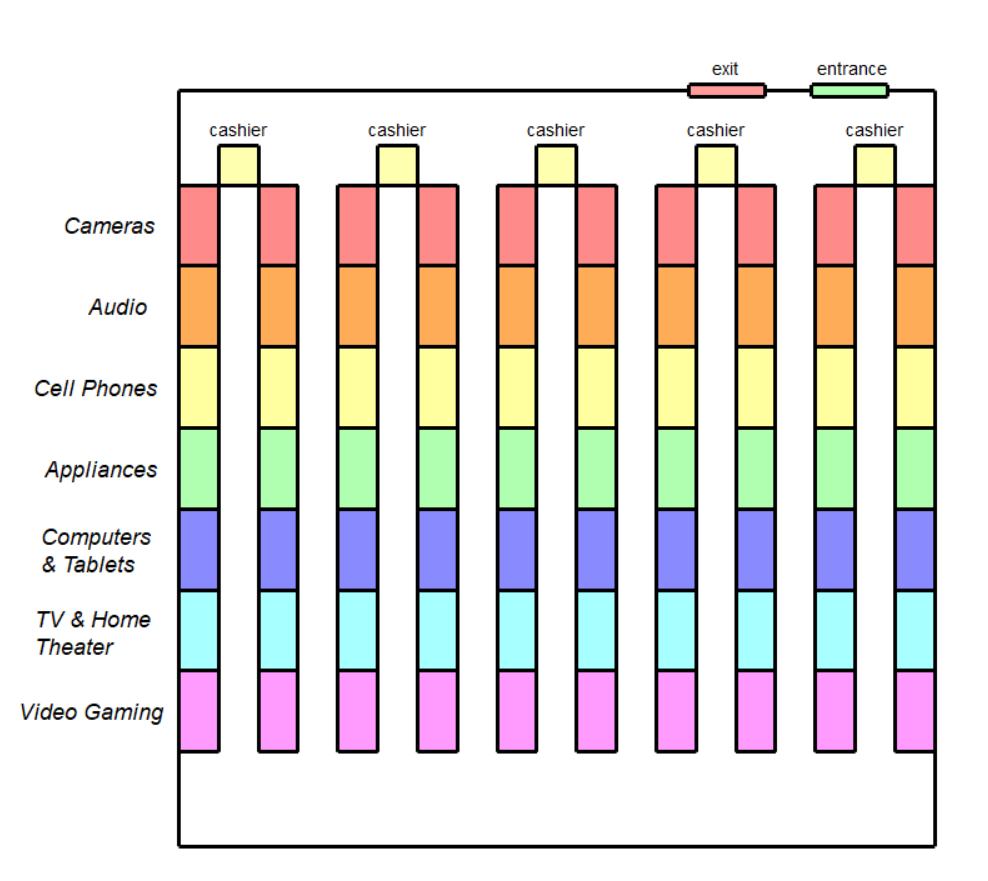
\includegraphics[width = 0.5\textwidth]{fig4.3.PNG}
\end{center}

From the picture, for each store block, the products will be placed only at the side adjacent to the walkway leading to the cashier. The other side would be just the wall leading customer to walk through the walkway to the bottom of the shopping hall.
Customers will enter at the entrance and walk into the space through the walkway between the wall, then make a u-turn into the space having the cashier at the end. They can pickup the products from here. 
The chaos inside the space containing the product would be less because the people are distributed into many groups and the walkway is straight.
The chaos at the entrance-exit area would be really bad but there's no products so there'll be no damage.
\newline

You can place the products according to the picture and the letter.
This would help minimize damage occured to your shop products and still give the same profit. 
\newline

Yours faithfully,\newline \par
Team 20200901.


\end{document}